\documentclass[12pt]{article}
\usepackage[margin=1in]{geometry}
\usepackage{amsmath, amsthm, amssymb, amsfonts, breqn, graphicx}

\theoremstyle{definition}
\newtheorem{problem}{Problem}
\renewcommand*{\proofname}{Solution}


\title{Homework Assignment 8}
\author{Matthew Tiger}


\newcommand{\E}{\text{E}}
\newcommand{\V}{\text{Var}}
\newcommand{\pdf}{\text{pdf}}
\newcommand{\pmf}{\text{pmf}}
\newcommand{\me}{\mathrm{e}}
\newcommand*\diff{\mathop{}\!\mathrm{d}}
\newcommand{\vect}[1]{\boldsymbol{#1}}
\newcommand{\norm}[1]{\left\lVert#1\right\rVert}


\begin{document}


\maketitle


% Problem 1
\begin{problem}
  Use uniform and Chebyshev nodes to interpolate
  \[
    f(x) = \frac{1}{1 + x^2},\ x \in [-5, 5].
  \]
  Using MATLAB, plot the graphs of $f(x)$ and the corresponding $P_n(f, x)$ for $n=10,20,40,80$.
\end{problem}

\begin{proof}
  The plots of the interpolating polynomial for the function $f(x) = 1 / (1+ x^2)$
  using uniform and Chebyshev nodes with $n$ sub-intervals for various values of
  $n$ can be found in the figure below.

  Make note of the large increases in scale as $n$ increases for the uniform nodes
  while the scale stays the same as $n$ increases for the Chebyshev nodes.
  Also note the near perfect agreement between $f(x)$ and the interpolating polynomial for large $n$ for Chebyshebv nodes.

  \begin{center}
    \makebox[\textwidth]{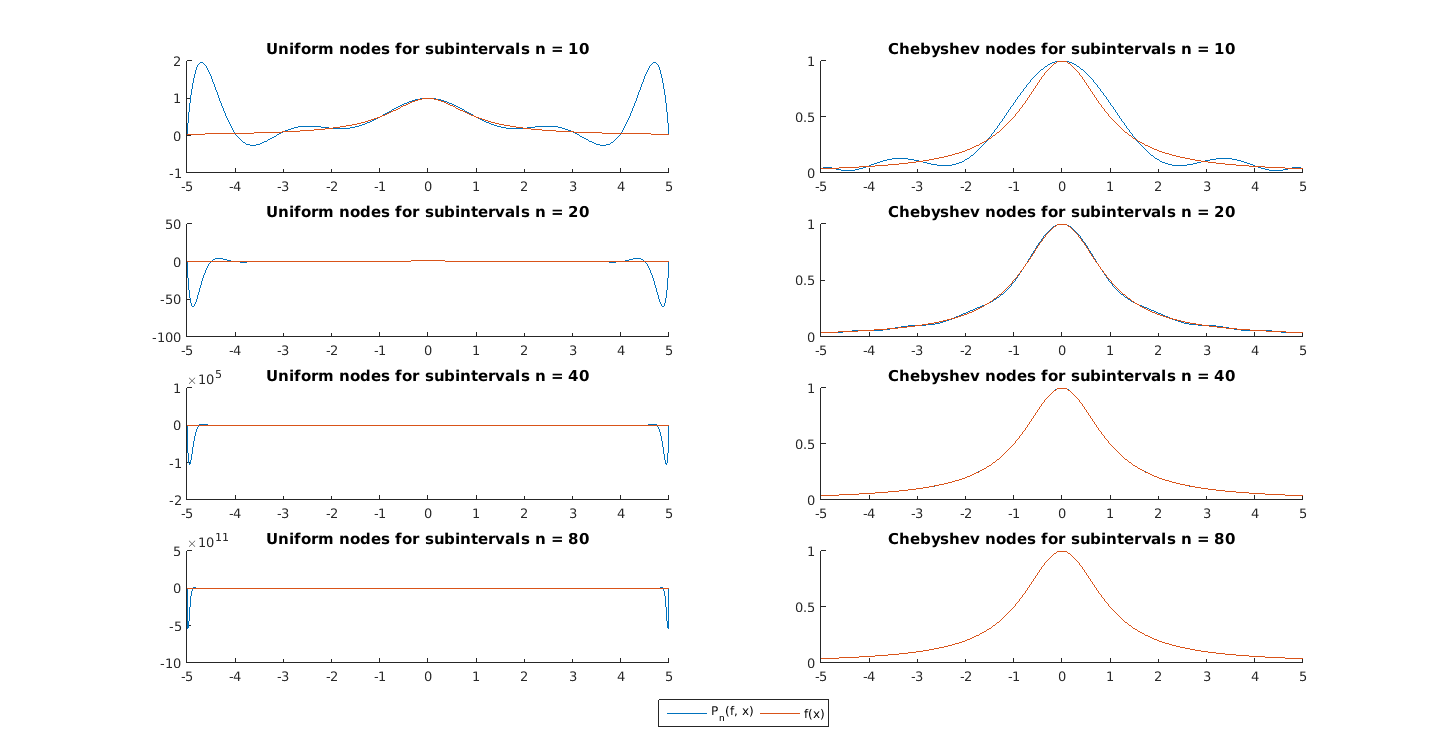
\includegraphics[width=\paperwidth]{./Interpolation/lagrange_polynomial_plot}}
  \end{center}
\end{proof}


% Problem 2
\begin{problem}
  Using MATLAB, code the Euler method for (12.7) on p. 285. Assume $\varepsilon = 0$.
  Plot your solutions for $n=10,20, $ and 40.
\end{problem}

\begin{proof}
  The figure below represents the solution to the first-order differential equation
  $y'(t) = -150 y(t) + 49 - 150 t$ for $t \in [0, 1]$ with initial condition $y(0) = 1/3$
  using Euler's method for $n$ sub-intervals for $n=10,20,$ and 40. Note that for $n=40$, we gain some additional data for the solution not present in other
  plots in the interval [0.9, 1].
  \begin{center}
    \makebox[\textwidth]{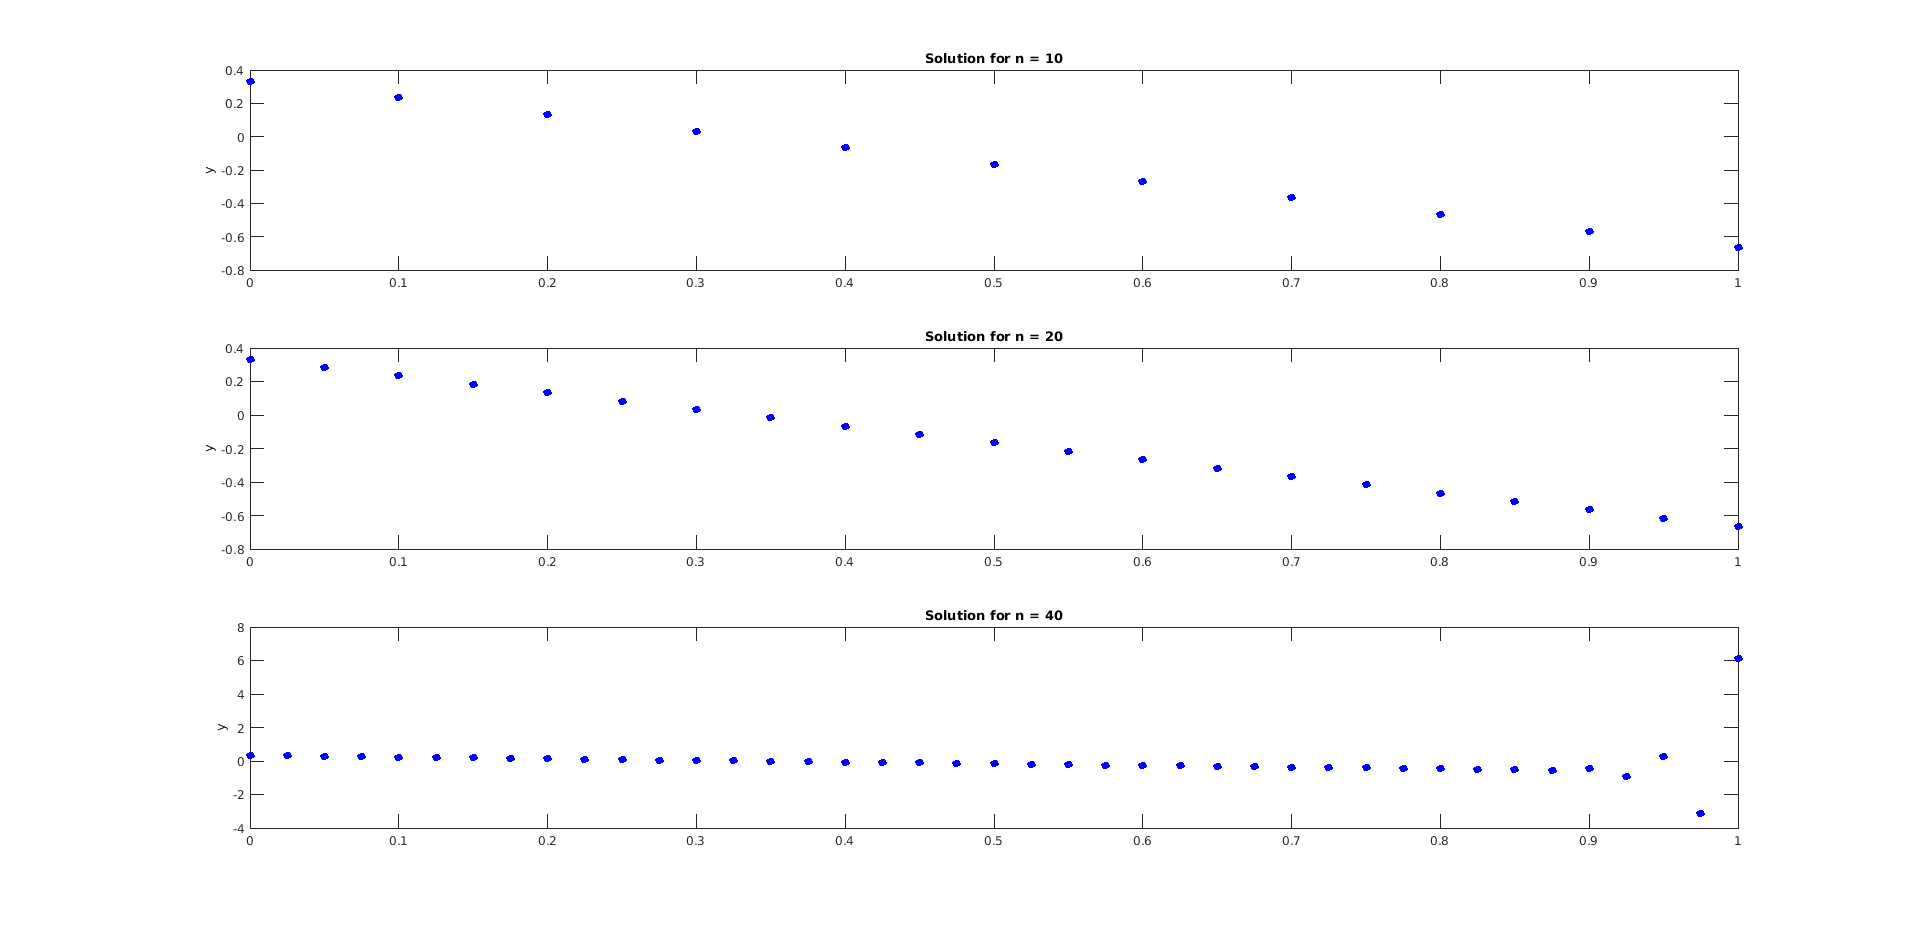
\includegraphics[width=\paperwidth]{./Euler/euler_plot}}
  \end{center}
\end{proof}


\end{document}
